
%(BEGIN_QUESTION)
% Copyright 2014, Tony R. Kuphaldt, released under the Creative Commons Attribution License (v 1.0)
% This means you may do almost anything with this work of mine, so long as you give me proper credit

Beregn $V_{AB}$ og $V_{CD}$ i denne kretsen, forutsatt at begge kildene og transformatorene har felles jord, og at begge transformatorene har viklingsforhold 1:1:

$$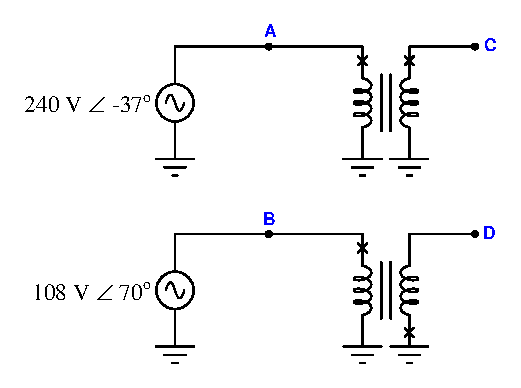
\includegraphics[width=15.5cm]{i00819x01.eps}$$

{\it Hint: siden alle transformatorene har viklingsforhold 1:1, må sekundærspenningen være identisk med primærspenningen for hver transformator. Det betyr at fasoren som representerer sekundærspenningen må ha nøyaktig samme lengde og vinkel som fasoren for den tilhørende primærspenningen. Behandle hver fasor som et linjestykke du kan flytte så lenge lengde og retning ikke endres, og se hvordan de ``stables'' i henhold til hvordan viklingene er elektrisk koblet i et komplett fasordiagram.}

\underbar{file i00819}
%(END_QUESTION)





%(BEGIN_ANSWER)

\noindent
{\bf Grafisk løsning (fasordiagram):}

$$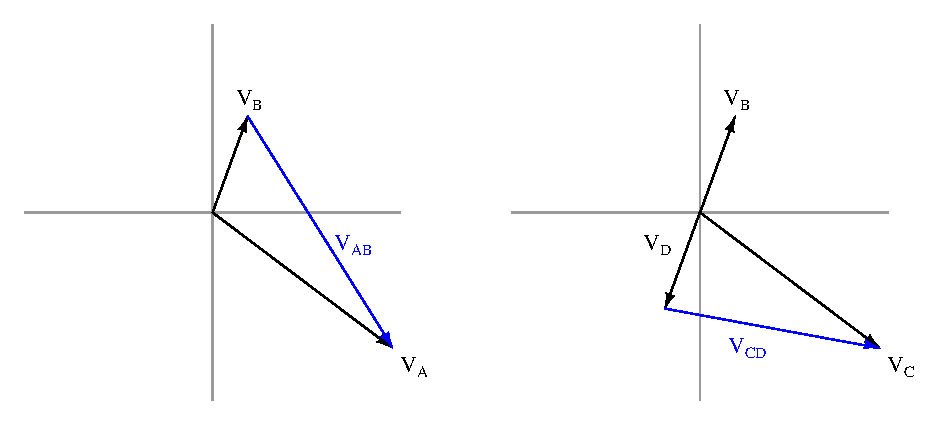
\includegraphics[width=15.5cm]{i00819x02.eps}$$

%(END_ANSWER)





%(BEGIN_NOTES)

\noindent
{\bf Symbolsk løsning:}

$$V_{AB} = V_A - V_B = (240 \hbox{ V} \angle -37^o) - (108 \hbox{ V} \angle 70^o) = 290.55 \hbox{ V} \angle -57.82^o$$

Merk at på grunn av direkte isolasjon i øvre transformator og faseinversjon i nedre transformator, blir $V_C = V_A$ og $V_D = - V_B$

$$V_{CD} = V_C - V_D$$

$$V_{CD} = V_A - (-V_B)$$

$$V_{CD} = V_A + V_B = (240 \hbox{ V} \angle -37^o) + (108 \hbox{ V} \angle 70^o) = 232.61 \hbox{ V} \angle -10.64^o $$






\vfil \eject

\noindent
{\bf Oppsummeringsquiz:}

Beregn spenningen mellom punkt B og D i denne kretsen ($V_{BD}$), forutsatt at begge kildene og transformatorene har felles jord og viklingsforhold 1:1:

$$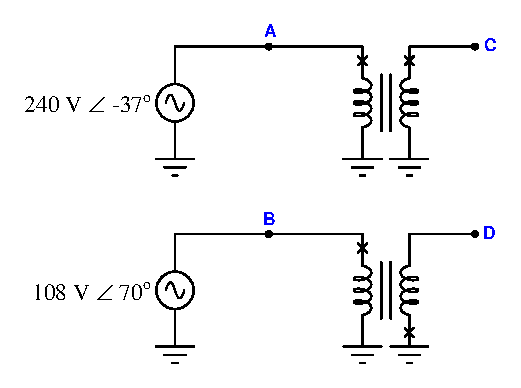
\includegraphics[width=15.5cm]{i00819x01.eps}$$

\begin{itemize}
\item{} 216.0 volt $\angle$ $70.0^o$
\vskip 5pt 
\item{} 240.0 volt $\angle$ $143^o$
\vskip 5pt 
\item{} 108.0 volt $\angle$ $-110^o$
\vskip 5pt 
\item{} 480.0 volt $\angle$ $-37.0^o$ 
\vskip 5pt 
\item{} 0.0 volt
\vskip 5pt 
\item{} 232.6 volt $\angle$ $-10.6^{o}$
\end{itemize}

%INDEX% Electronics review: AC transformer circuit
%INDEX% Electronics review, phasor expressions of circuit quantities

%(END_NOTES)
